\chapter{Perancangan}
\label{chap:perancangan}
Bab ini akan membahas mengenai perancangan perangkat lunak berdasarkan hasil analisis pada Bab \ref{chap:analisis}. Bab ini mencakup perancangan kelas, perancangan antar muka, dan perancangan protokol.
\section{Perancangan Kelas}
\label{sec:rancangandiagramkelas}

\begin{figure}[H] 
    \centering  
    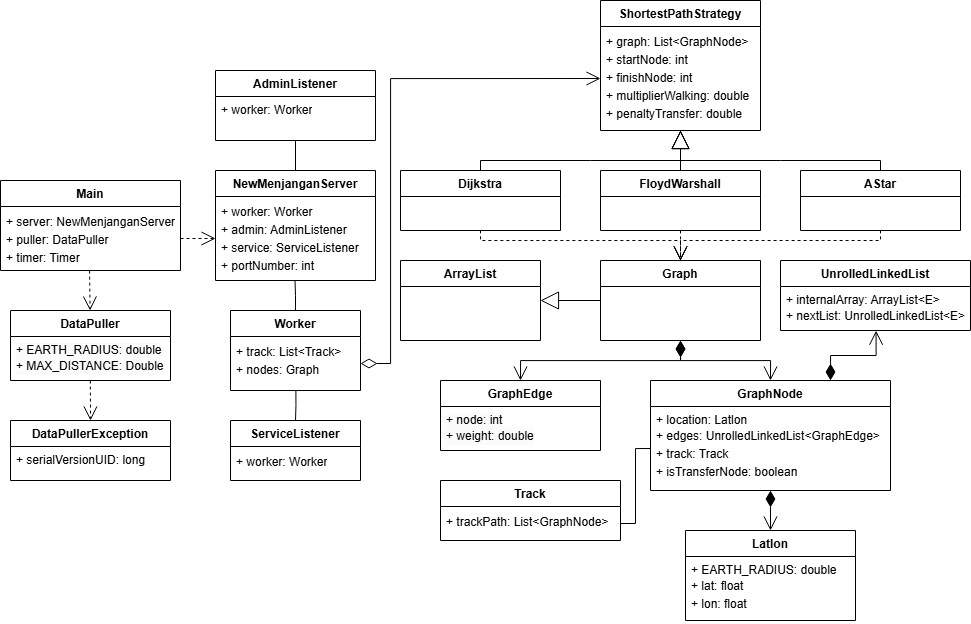
\includegraphics[width=1\textwidth]{class-diagram-2}  
    \caption{Perancangan Kelas}
    \label{fig:rancangandiagramkelas} 
\end{figure}

\noindent
Perancangan kelas dilakukan untuk merepresentasikan struktur perangkat lunak setelah dilakukan pengembangan terhadap peran KIRI. Perubahan ini difokuskan pada penerapan Strategy Pattern guna meningkatkan fleksibilitas sistem dalam menggunakan berbagai algoritma pencarian jalur terpendek. Gambar \ref{fig:rancangandiagramkelas} menunjukkan struktur kelas setelah pengembangan dilakukan.
\\
Sebelumnya, algoritma shortest path diimplementasikan secara langsung dalam sistem menggunakan algoritma Dijkstra. Oleh karena itu, dilakukan perubahan desain dengan menerapkan Strategy Pattern dengan dibuatnya kelas abstrak ShortestPathStrategy yang menjadi dasar dari semua algoritma shortest path. Kelas-kelas seperti Dijkstra, FloydWarshall, dan AStar kemudian diimplementasikan sebagai turunan dari ShortestPathStrategy. Dengan struktur ini, ketiga algoritma tersebut dapat saling dipertukarkan tanpa memengaruhi bagian lain dari sistem, karena semuanya mengikuti superclass-nya, yaitu ShortestPathStrategy. Strategi ini memudahkan sistem dalam memilih dan menggunakan algoritma pencarian jalur terpendek yang sesuai dengan kebutuhan tertentu. Selain itu, Struktur kelas seperti GraphNode, GraphEdge, dan Graph tetap dipertahankan, namun kini berfungsi mendukung berbagai algoritma.
\\
Kelas ShortestPathStrategy memiliki atribut-atribut yang sebelumnya terdapat pada Dijkstra, yaitu graph, startNode, finishNode, multiplierWalking, dan penaltyTransfer. Atribut-atribut tersebut akan diturunkan dan digunakan oleh seluruh algoritma shortest path. Selain itu, kelas ShortestPathStrategy juga memiliki method-method yang di-override dari kelas-kelas algoritma shortest path.
\\
Dengan perancangan ini, perangkat lunak KIRI kini memiliki arsitektur yang lebih modular dan akan lebih mudah apabila akan dikembangkan lebih lanjut, baik dari sisi algoritma maupun fungsionalitas lain.


\section{Perancangan Antarmuka}
\label{sec:rancanganui}

\begin{figure}[H]
    \centering
    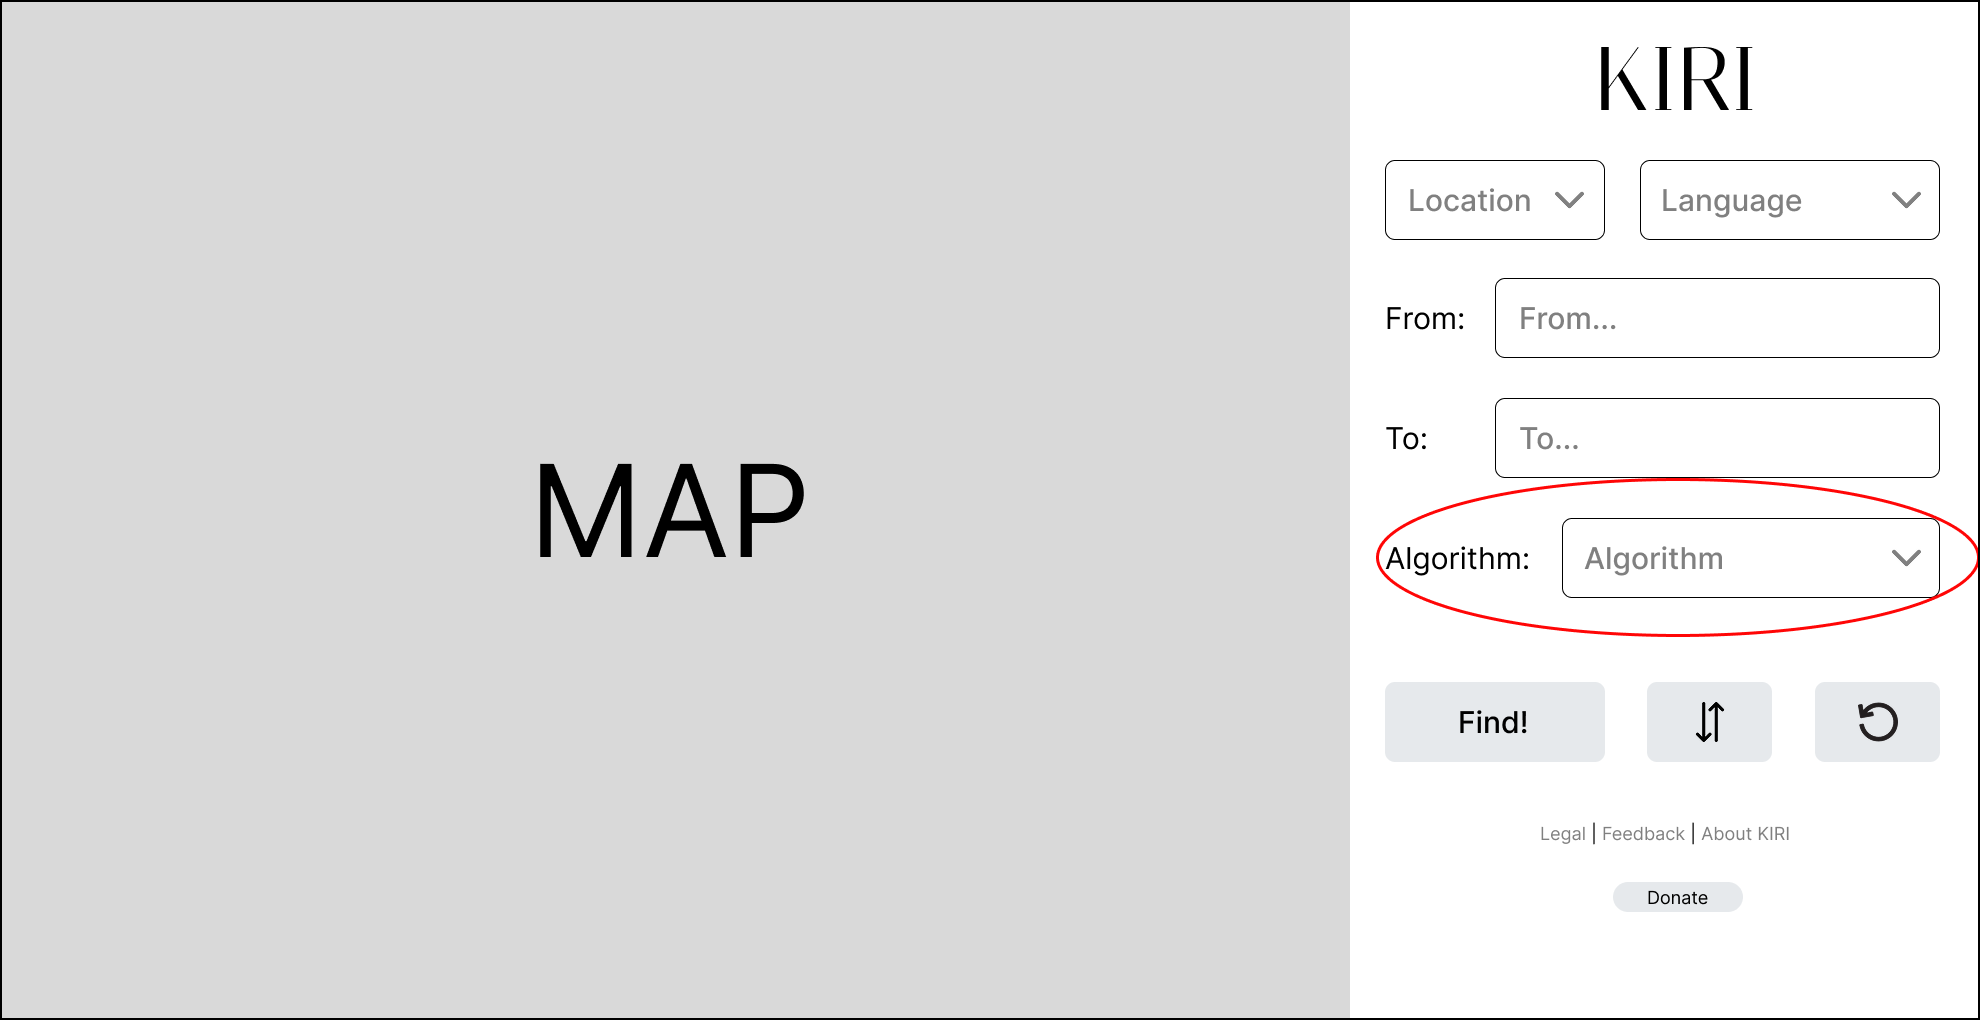
\includegraphics[width=1.1\textwidth, height=1\textheight, keepaspectratio]{rancangan-ui}
    \caption{Rancangan Antarmuka}
    \label{fig:rancanganui}
\end{figure}

\noindent
Dilakukan sedikit perubahan pada halaman antarmuka dari perangkat lunak KIRI, yaitu dengan menambahkan sebuah \textit{dropdown} baru untuk memilih algoritma yang akan digunakan, seperti pada gambar \ref{fig:rancanganui}. Pada \textit{dropdown} tersebut akan terdiri dari 3 buah algoritma \textit{shortest path} yang sudah diimplementasikan sebelumnya, yaitu Dijkstra, Floyd-Warshall, dan A-Star. 
\newpage
\section{Perancangan Protokol}
Dilakukan sedikit modifikasi pada protokol API untuk memberikan fleksibilitas pengguna dalam memilih algoritma jalur terpendek yang akan digunakan, seperti Dijkstra, A*, dan Floyd-Warshall. Modifikasi dilakukan pada bagian \textit{front-end} (Tirtayasa) dan juga \textit{back-end} (NewMenjangan). Perubahan ini hanya menambah satu parameter baru tanpa mengubah struktur data utama sehingga modifikasi dapat dilakukan tanpa mempengaruhi fungsi sistem lainnya secara signifikan.

\subsubsection{Tirtayasa}
Pada bagian ini akan dilakukan modifikasi pada protokol API, yaitu akan dilakukan modifikasi pada kode-kode program yang berkaitan dalam pengiriman data ke bagian \textit{back-end}. Berikut merupakan kode-kode program yang akan modifikasi.
\begin{itemize}
    \item \textbf{main.js}
    \\ Pada kode ini modifikasi yang akan dilakukan adalah penambahan parameter baru pada \textit{function} \texttt{checkCoordinatesThenRoute} ketika akan memanfaatkan \textit{function} \texttt{findroute} akan ditambahkan sebuah parameter baru yang akan mengirimkan algoritma yang dipilih.

    \item \textbf{protocol.js}
    \\ Pada kode ini modifikasi yang akan dilakukan adalah penambahan parameter baru pada saat mendefinisikan \textit{function} \texttt{findroute} yaitu parameter untuk algoritma yang dipilih.

    \item \textbf{Api.php}
    \\ Pada kode ini modifikasi yang akan dilakukan adalah penambahan parameter baru pada \textit{function} \texttt{\_findroute} yaitu parameter untuk algoritma yang dipilih.
\end{itemize}

\subsubsection{NewMenjangan}
Pada bagian ini akan dilakukan modifikasi pada kelas yang akan menerima parameter-parameter yang dikirimkan dari bagian Tirtayasa. Berikut merupakan kelas yang akan modifikasi.

\begin{itemize}
    \item \textbf{ServiceListener.java}
    \\ Pada kelas ini modifikasi yang akan dilakukan adalah penambahan parameter baru, yaitu parameter untuk algoritma yang dipilih.
\end{itemize}